\documentclass[10pt,twocolumn,letterpaper]{article}

\usepackage{cvpr}
\usepackage{times}
\usepackage{epsfig}
\usepackage{graphicx}
\usepackage{amsmath}
\usepackage{amssymb}
\usepackage{float}
\usepackage{caption}


% Include other packages here, before hyperref.

% If you comment hyperref and then uncomment it, you should delete
% egpaper.aux before re-running latex.  (Or just hit 'q' on the first latex
% run, let it finish, and you should be clear).
\usepackage[breaklinks=true,bookmarks=false]{hyperref}

\cvprfinalcopy 

\def\httilde{\mbox{\tt\raisebox{-.5ex}{\symbol{126}}}}


\graphicspath{ {images/} }


\setcounter{page}{1}
\begin{document}

%%%%%%%%% TITLE
\title{Spotting Distracted Drivers Using Classic CV Methods}

%%%%%%%%% Author Names
\author{Guillermo Reyes\\
{\tt\small enggreys@gmail.com}
\and
Daniel Schaefer\\
{\tt\small s9dlscae@stud.uni-saarland.de}
\and
Marc Tonsen\\
{\tt\small secondauthor@i2.org}
\and
Dominik Weber\\
{\tt\small secondauthor@i2.org}
}

\maketitle

%%%%%%%%% ABSTRACT
\begin{abstract}
   In this project we tried to solve the task of deciding whether or not a driver is distracted, and if so, what the driver is being distracted by. For this we explored the possibilities of classical computer vision algorithms instead of using Deep Learning mainly because of computational limitations and already publicly available solutions using Deep Learning.
\end{abstract}

%%%%%%%%% BODY TEXT

\section{Introduction}


According to the U.S. Department of Transportation and National Highway Traffic Safety Administration, about 18\% of all injury crashes and 10\% of fatal crashes are reported to involve distracted drivers at the moment of the accident ~\cite{knuthwebsite}. In 2013 this, unfortunately, translated to over 3000 people killed and 400,000 people injured, in the United States alone due to motor vehicle crashes.

This clearly speaks for measures to be taken. Spotting distracted drivers in time could help to take appropriate actions and thus prevent accidents and save thousands of lives every year. In order to detect distracted drivers, different approaches have been taken. However, many of them are intrusive and expensive. However by using simple cameras combined with computer vision algorithms, one can get a solution that is both cheap and non-intrusive.\\

For this task we have entered the Kaggle Competition: State Farm Distracted Driver Detection ~\cite{Kaggle}. The challenge consists of classifying images of drivers engaging in the behaviors described below.

\begin{enumerate}
	\item Safe driving
	\item Texting with right hand
	\item Talking on the phone with right hand
	\item Texting with left hand
	\item Talking on the phone with left hand
	\item Operating the radio
	\item Drinking
	\item Reaching behind
	\item Hair and makeup
	\item Talking to passenger
\end{enumerate}

In this paper we propose different approaches to solve this task using some classic computer vision methods to find out how well they stack up against state of the art methods such Deep Neural Networks, which can already achieve up to 99\% accuracy .

% TODO erwaehnen von Computational Limits + allgemein gruende fuer die entscheidung kein cnn zu machcen


\section{Related Work}

There are already quite a few approaches regarding distracted driver distraction, although these approaches are mainly working on picture datasets with frontal-views on the face and rely almost exclusively on gaze-tracking or head-pose estimation. \cite{Dorazio} \cite{6957817}

Additionally some of these datasets are being captured in artificial environments (for example Racing Simulators) \cite{itsc:bergasa2008} which results in much more consistent variables like e.g. light situation and camera angle. In some of the approaches additional sensors are being used (e.g. RGB-depth cameras) which obviously also extend the possibilities greatly but also the cost is increased. \cite{Ragab2014}

We also decided to do some research on the very familiar topic ''Activity Recognition'' to explore further possibilities. Unfortunately most of the approaches in the Activity Recognition field rely on additional sensors (eg. wearable sensors) \cite{6258525} \cite{6365160} or rely on continuous video instead of single pictures. \cite{1315249} \cite{1430826}

We conclude that current methods are not completely applicable to the problems we have at hand, so we have to come up with something new.




\section{The Dataset}
The first step we took was analyzing the dataset. We are given over 2.000 pictures per class from 26 different drivers in total. Each of the drivers has roughly the same amount of pictures per class. 

The drivers are split up in four cars. Depending on the car the camera angles varies. During the analysis process we also noticed that there is labeling noise in the data. For example we found several pictures in the ''safe driving'' class, which should in our opinion belong to the ''Talking to passenger'' one. Also lighting-conditions changed rapidly and the drivers have different ethnicities.


Additionally to this so called training set, of which we know the driver (and thus car) and class of each picture, we also have a so called test set containing around 80.000 unclassified pictures. The only option to verify results on this set is to upload them to the competition website, but because of the time necessary to classify all these 80.000 pictures combined with the fact that we only get very limited information back, we decided to run our tests only on parts of the training set to speed up our evaluation process.



\section{Proposed Methods}
In this paragraph we are going to explain the different approaches we had in mind.

\subsection{Head-based classification}
\begin{figure}[h]
	\centering
	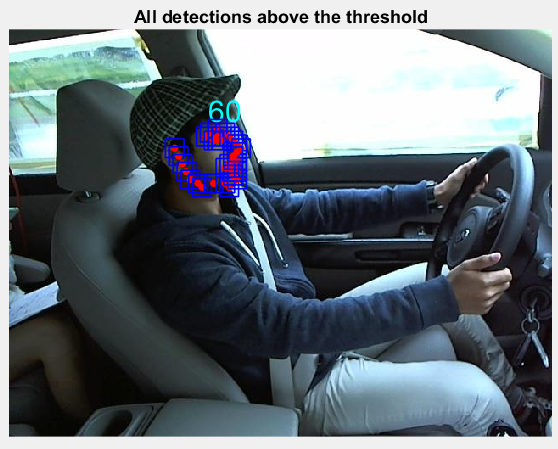
\includegraphics[width=0.2\textwidth]{face1}\hspace{0.01\textwidth}
	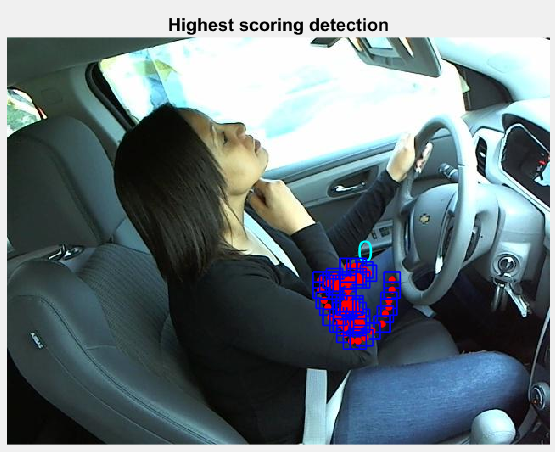
\includegraphics[width=0.2\textwidth]{faces/face7}\\ \vspace{0.01\textwidth}
	\caption{good and bad example of Face}
	\label{face_estimation_example}
\end{figure}
One of our ideas was to use a head-detector or a face-detector to extract a feature and predict the correct class or narrow down the possible classes. At least we hoped it would be possible to say if a picture is in a specific class or not. We tried different head or face-detectors and all had Problems to detect the head or didn't gave us enough features. We think the problem was that the pictures have a relative small resolution. An other Problem could be the different angles, because some detectors only worked with frontal view others only in the side view. Long hair, sunglasses and other occlusion could be a problem too. In the end we found Face~\cite{Ramanan:2012:FDP:2354409.2355119}, which found heads in about 80\% of the pictures and gave us the horizontal angle from face to camera and 39 or 68 points of the face.Even if it found a face, it was not always the correct one. Face is running in matlab, so we used it to create a .csv file for every class + a file for the pictures where it was impossible to find a head. Then we let a Support Vector Machine and a Random learn on this data. First we only used the angle. Then we used angle and the points in relation to a fixed point in the face and hoped that these point could show us if the person is looking straight or looking down on his mobile phone or the radio. We tried with both to predict the right class and to predict if the person is talking to the passenger or not.


\subsection{Hand-based classification}
\begin{figure}[h]
	\centering
	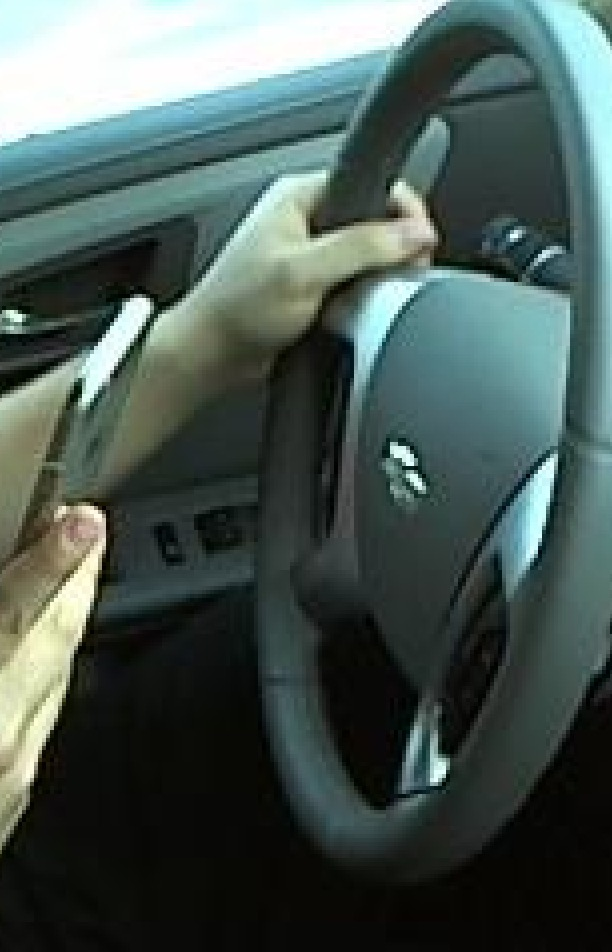
\includegraphics[width=0.2\textwidth]{handpose_example_1_cut}\hspace{0.01\textwidth}
	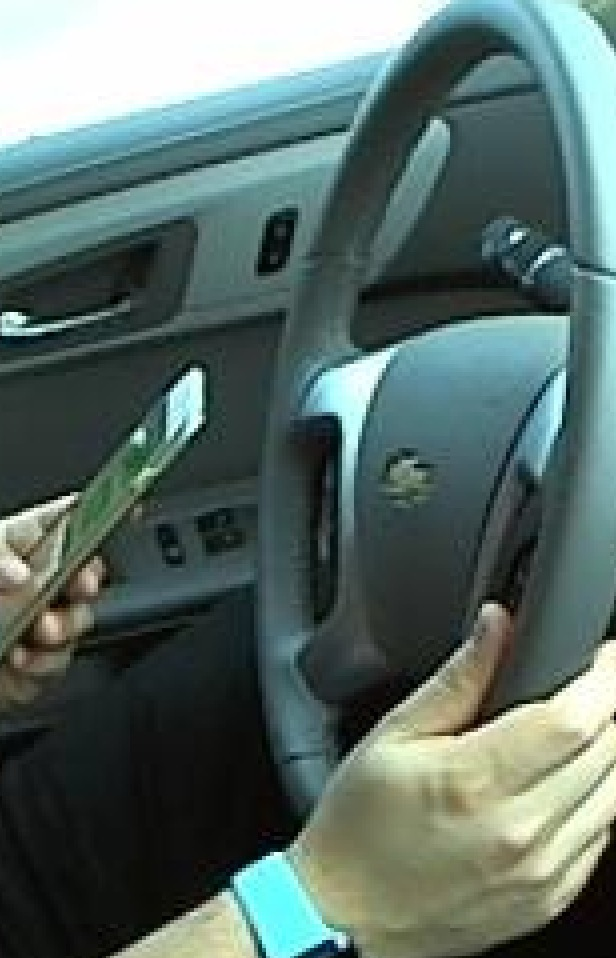
\includegraphics[width=0.2\textwidth]{handpose_example_2_cut}\\ \vspace{0.01\textwidth}
	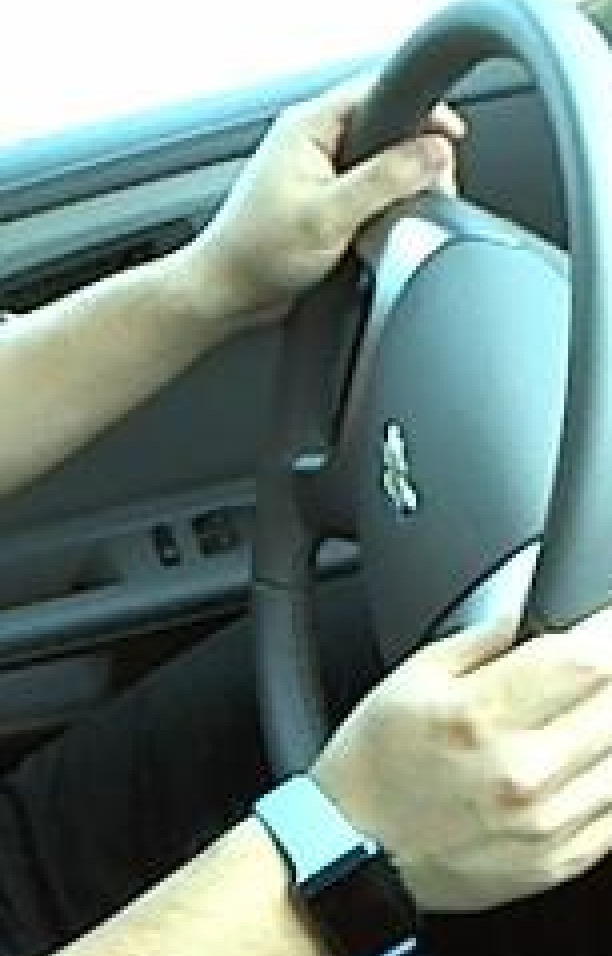
\includegraphics[width=0.2\textwidth]{handpose_example_3_cut}\hspace{0.01\textwidth}
	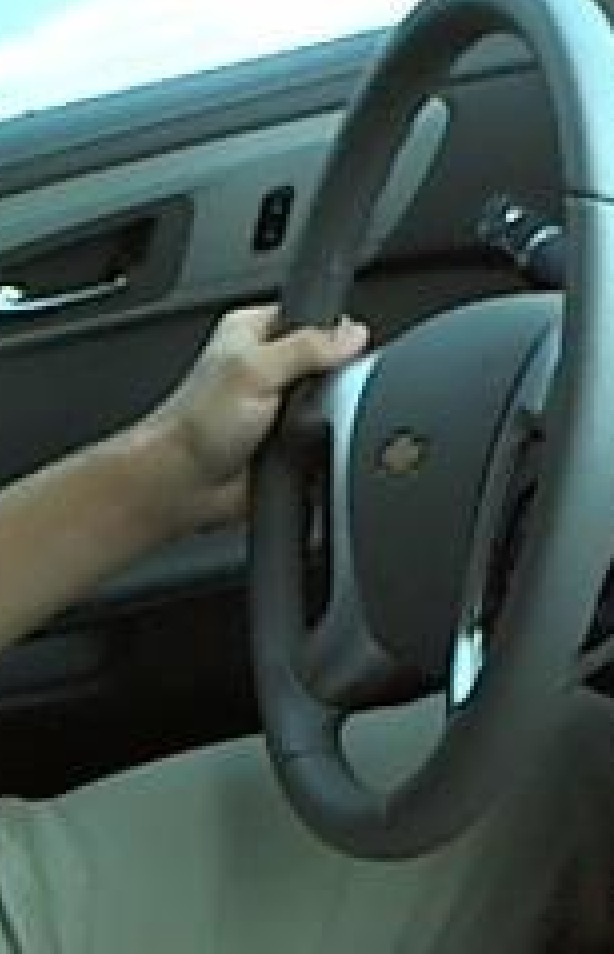
\includegraphics[width=0.2\textwidth]{handpose_example_4_cut}
	\caption{Examples of the cropped images we are using to train a classifier. The classes of the images from top-left to bottom-right are: Texting Right, Texting Left, Safe Driving, Reaching behind.}
	\label{hand_estimation_example}
\end{figure}
When examining the dataset, we found that many of the classes can be well distinguished when only considering the part of the image in the vicinity of the steering wheel. All of the activities described by the different classes in the task are performed with the arms, therefore their appearance is a strong indicator of the corresponding class. Based on this, we have cropped the images in the dataset to a fixed size of 155x240 px, to only contain the steering wheel and its immediate surroundings. See Fig. \ref{hand_estimation_example} for an illustration of those images and to see an example of how well some classes can be distinguished from that partial image. On those images we have trained a classifier to distinguish all classes and some to solve a 1-vs-1 classification task between only two classes. We have also tried to segment the classes into clusters and to classify based on those clusters, but our results were not satisfactory and we will not discuss this approach further. We have tried out different features for the classification:
\begin{itemize}
	\item \textbf{Raw Image}: We use a raw downscaled version of the image as a feature.
	\item \textbf{HoG}: Histogram of oriented gradients, which we have discussed in the lecture. We use the scikit-image implementation
	\item \textbf{LBP}: Local binary patterns, which is a feature originally developed for texture classification. It has been reported to work well in combination with HoG features in some cases. We also use the scikit-image implementation for this.
\end{itemize}
Besides using Support Vector Machines for classification, which was the only classifier discussed in the lecture, we have also tried Random Forrests.\\
It is important to note that the steering wheel is not aligned across the dataset. The training-data was recorded in 4 different cars with varying camera angles. As we will show, it is important to align the steering wheel in the cropped images for a good performance. We have manually labeled the center of all steering wheels to perform this alignment.



\subsection{Bodepose-based classification}
We expected that reliable localization of head and arms would allow us to differentiate most of the classes because of the different positions the mentioned body-parts are in, during the different distractions.

On gitHub we found the open source implementation ''Convolutional Pose Machines'' which is able to predict the key bodyparts for us, like wrists, shoulders, elbows, neck and head.\cite{DBLP:journals/corr/WeiRKS16} The paper was presented at the Conference on Computer Vision and Pattern Recognition in 2016 and outperformed everything else we found greatly using the pretrained models provided on gitHub. 

Unfortunately we could not use this implementation in our project, because of the computational performance necessary. Nobody of us had access to a CUDA supported video card with over two gigabytes of VRAM which was not nearly enough for this Pose-Machine to work. Doing everything on CPU was not an option for us because this took between one to four minutes per picture. Although this at least made it possible to take a look at the results this pose machine is able to achieve using neural networks. We can not really precisely evaluate the performance of this approach but in all the pictures we were able to test the heatmaps of the said body-parts are looking usable across all the different classes. You can see an example of how the heatmaps for interesting bodyparts look like in Figure \ref{BodyPoseExample}.\\
\begin{figure}[h]
    \centering
    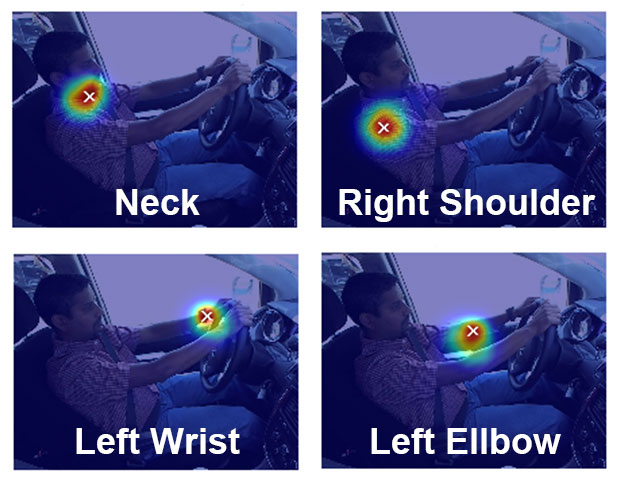
\includegraphics[width=0.5\textwidth]{BodyPoseExample}
    \caption{Example Heatmaps of Conbolutional Pose Machines}
    \label{BodyPoseExample}
\end{figure}

Without our computational limitations these bodypose-machines would probably be a very nice addition to the headpose and handpose estimation we are currently using.


\subsection{HOG Landmarks}

For the last approach used in this paper, we look for specific things in the images that help us make a decision. We call these specific things landmarks. A landmark can be anything in the images(pose, objects, etc.) that can be used to distinguish a class from the others. These landmarks are chosen arbitrarily in this paper and we shall later evaluate how well they perform. Below we outline what of these landmarks are, note that there is at least one distinctive landmark per class.

\begin{enumerate}
	\item Head facing front, towards the road.
	\item Head facing sideways towards the copilot
	\item Head facing backwards towards the back passengers.
	\item Empty gap in front of the head rest
	\item Right hand holding phone while texting
	\item Right hand holding phone while talking\
	\item Left hand holding phone while texting
	\item Left hand holding phone while talking
	\item Hand holding bottle/cup
	\item Hand scratching near head
	\item Hand reaching behind
	\item Hand reaching for radio	
\end{enumerate}


\begin{figure}[h]
	\centering
	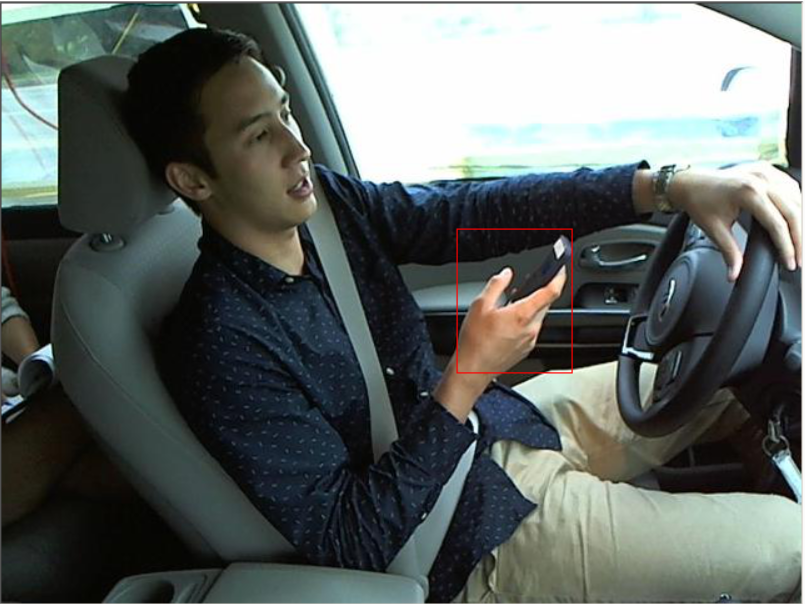
\includegraphics[width=0.45\textwidth]{mult_HOG/HOG_phone_det}%\vspace{0.01\textwidth}
%	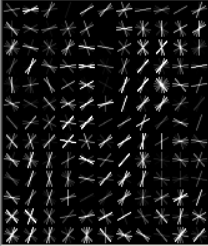
\includegraphics[width=0.25\textwidth]{mult_HOG/HOG_phone}
	\caption{Bounding box around phone on the right hand while texting. }
	\label{HoG_phone_det}
\end{figure}

\begin{figure}[h]
	\centering
	%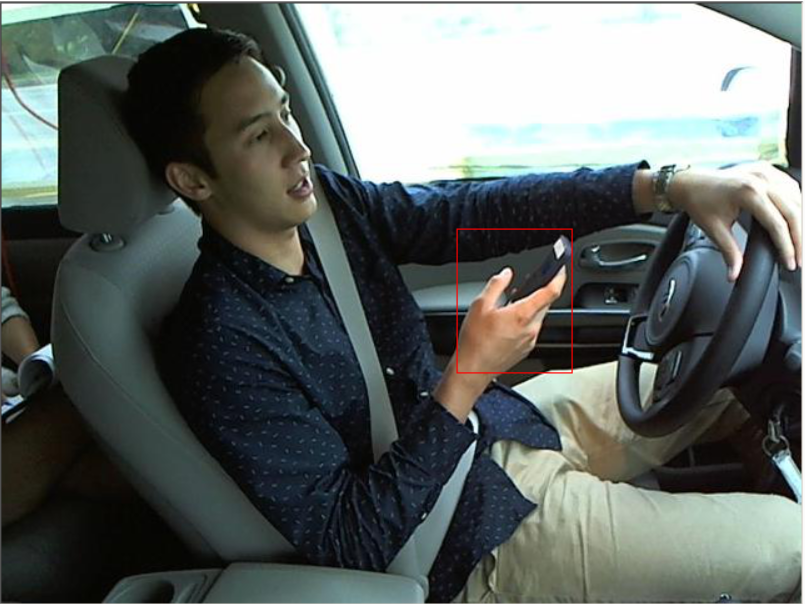
\includegraphics[width=0.45\textwidth]{mult_HOG/HOG_phone_det}%\vspace{0.01\textwidth}
		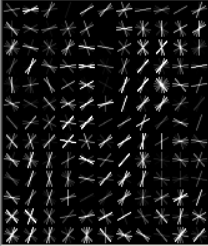
\includegraphics[width=0.25\textwidth]{mult_HOG/HOG_phone}
	\caption{HoG of the right hand holding phone while texting landmark after training with approximately 50 images}
		\label{HoG_phone}
	\end{figure}

In order to detect this landmarks, approximately 50 images per class were taken and manually labeled bounding boxes around the selected landmarks. The detectors were then trained based on HoG features for each landmark with the help of Dlib \cite{dlib09}. In Figure \ref{HoG_phone_det} one can see an example of a detection of a person texting with the right hand, and in Figure \ref{HoG_phone} what the HoG for this landmarks looks like.

After having trained the detectors, one can use these to determine whether a certain landmark is present in an image or not. Then, by training a simple SVC that uses as predictors an array of boolean features each one of which representing the presence, or absence, of a landmark, one can potentially predict the activity performed by the driver.



 



%\begin{minipage}[t]{.5\textwidth}
%	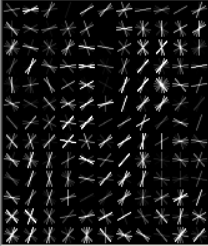
\includegraphics[width=\textwidth]{mult_HOG/HOG_phone}
%	\captionsetup{justification=raggedright, singlelinecheck=false}
%	\captionof{figure}{H Feistel Function}
%\end{minipage}%
%\begin{minipage}[t]{.5\textwidth}
%	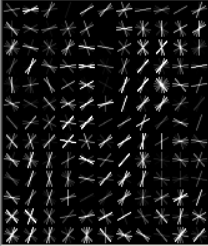
\includegraphics[width=\textwidth]{mult_HOG/HOG_phone}
%	\captionsetup{justification=raggedright, singlelinecheck=false}
%	\captionof{figure}{HOG of the right hand holding phone while texting landmark}
%\end{minipage}


%\begin{figure*}[h]
%	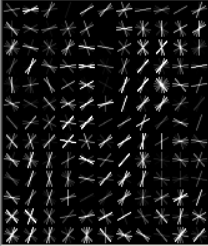
\includegraphics[width=0.85\columnwidth]{mult_HOG/HOG_phone}
%	\captionsetup{justification=raggedright,
%		singlelinecheck=false
%	}
%	\caption{HOG of the right hand holding phone while texting landmark}
%\end{figure*}





\section{Experimental Results}
Listing of the results we could achieve using the headpose estimation and the hand-based classification and finally the HoG landmarks.
\subsection{Headpose Estimation}
	\subsubsection{Angle as feature}
	Out first try was to only use the angle of the face to the camera as a feature. The results(Figure\ref{headpose_feature}) were bad. The Problem was that the angle alone was far to less information.
	\begin{figure}[h]
	\centering
	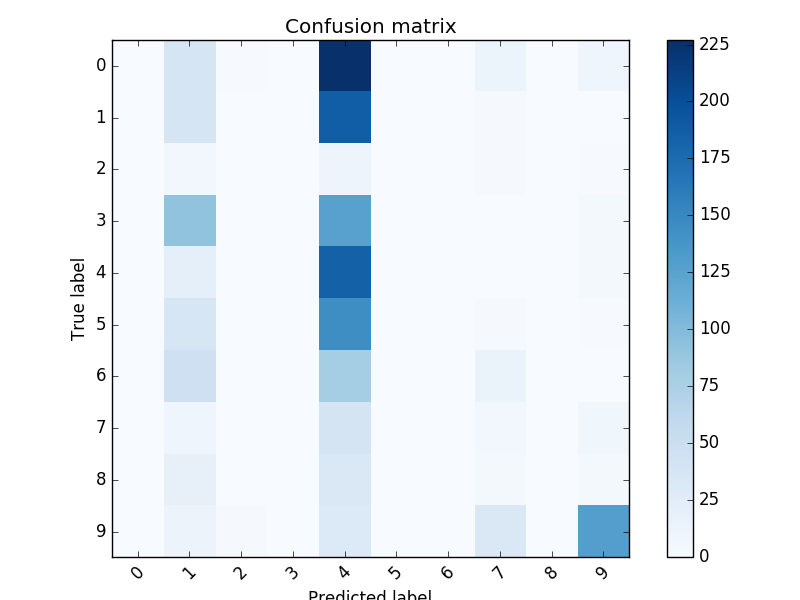
\includegraphics[width=0.5\textwidth]{angle_only}\hspace{0.01\textwidth}
	\begin{tabular}{c||c|c|c|c}
	  & precision&recall&f1-score&support\\	\hline
	 c0&0.00&0.00&0.00&288\\
	 c1&0.12&0.17&0.14&227\\
	 c2&0.00&0.00&0.00&20\\
	 c3&0.00&0.00&0.00&222\\
	 c4&0.17&0.88&.029&210\\
	 c5&0.00&0.00&0.00&184\\
	 c6&0.00&0.00&0.00&142\\
	 c7&0.09&0.11&0.10&65\\
	 c8&0.00&0.00&0.00&59\\
	 c9&0.80&.062&0.70&208
	\end{tabular}
	\caption{results of angle features with svm}
	\label{headpose_feature}
	\end{figure}
\subsubsection{Angle and points as features}
\begin{figure}[h]
	\centering
	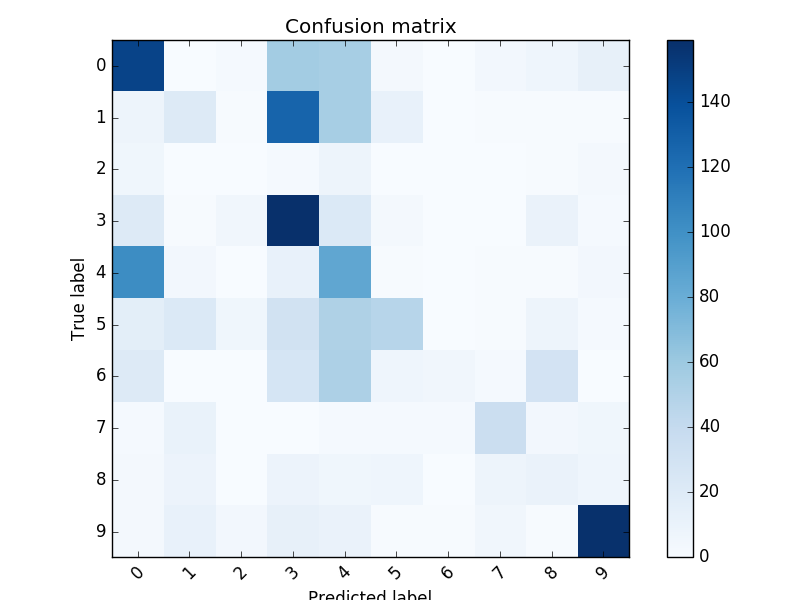
\includegraphics[width=0.5\textwidth]{all_vs_all_headpose}\hspace{0.01\textwidth}
	\begin{tabular}{c||c|c|c|c}
	  & precision&recall&f1-score&support\\	\hline
	 c0&0.45&0.51&0.48&288\\
	 c1&0.26&0.09&0.14&227\\
	 c2&0.00&0.00&0.00&20\\
	 c3&0.36&0.72&0.48&222\\
	 c4&0.25&0.40&0.31&210\\
	 c5&0.57&0.26&0.51&84\\
	 c6&0.62&0.04&0.07&142\\
	 c7&0.62&0.55&0.59&65\\
	 c8&0.14&0.17&0.15&59\\
	 c9&0.81&0.76&0.78&208
	\end{tabular}
	\caption{results of angle and points features with svm}
	\label{headposeandpoints_feature}
	\end{figure}
Our next idea was to use the points of the face in relation to a fixed point in the face in the hope that it would help us to recognise the vertical angle of the drivers head. The results(Figure\ref{headposeandpoints_feature}) were a little bit better ut still far from good.

\subsubsection{one vs. all with head-pose and points}
\begin{figure}[h]
	\centering
	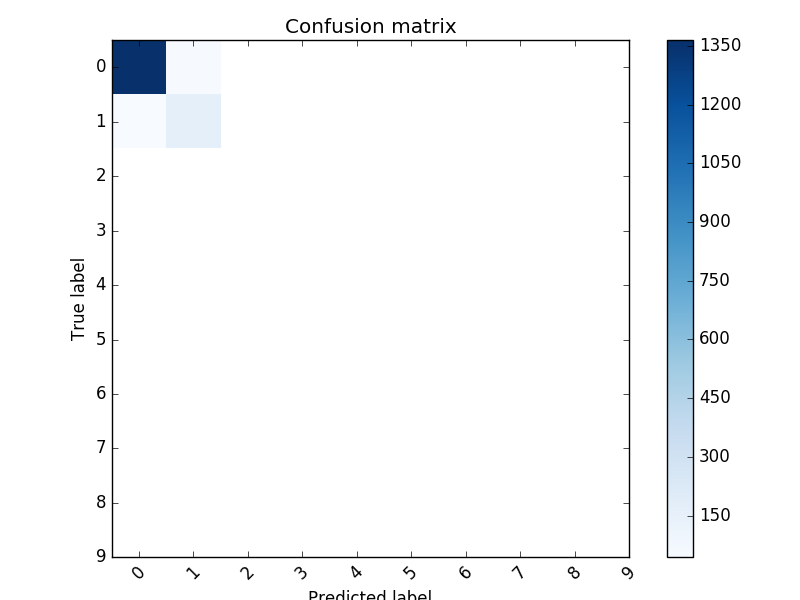
\includegraphics[width=0.5\textwidth]{c5ornot.png}\hspace{0.01\textwidth}
	\begin{tabular}{c||c|c|c|c}
	  & precision&recall&f1-score&support\\	\hline
	  not C5&0.97&0.96&0.97&1417\\
	  C5&0.76&0.79&0.78&208
	\end{tabular}
	\caption{results of angle and points features with svm}
	\label{C5ornot}
	\end{figure}
Our last try was to test if it is possible to find out if the image is in the class ``talking to the passenger'' or not. Again we trained with angle and relative points, but this time only C5 and notC5. The results(Figure\ref{C5ornot}) were better bur not satisfiable, because it is still too bad to use it in the project.

\subsection{Hand-based classification}

	\subsubsection{Alignment of the steering wheel}
	\begin{table}
		\begin{tabular}{c|c|c}
			Within 1 car & No alignment & With alignment \\ 
			\hline 
			37\% & 10\% & 24\% \\ 
		\end{tabular} 
		\caption{Average classification accuracies for different levels of steering wheel alignment.}
		\label{hand_estimation_alignment}
	\end{table}
	
	To investigate the impact of image alignment we have trained classifiers on 3 different sets of data:
	\begin{itemize}
		\item 11 participants recorded in the same car and with the same camera angle, who are therefore perfectly aligned
		\item Unaligned crops from all participants, i.e. a window with a fixed size and position
		\item Aligned crops from all participants based on our labellings of the steering wheel
	\end{itemize}
	As one can see in Table \ref{hand_estimation_alignment} alignment significantly improves the results. The results on data coming from only a single car can be regarded as an upper limit with 37\% accuracy. With no alignment the accuracy was only 10\% which is equal to random guessing, while the accuracy was 24\% with alignment. For all further experiments the steering wheels were therefore aligned.


	\subsubsection{Feature evaluation}
	\begin{table}
		\begin{tabular}{c|c|c|c|c}
			& Raw & HoG & LBP & HoG+LBP \\ 
			\hline 
			SVR & 25\% & 32\% & 23 \% & n.A. \\ 
			\hline 
			Random Forest & 27\% & 26\% & 16\% & n.A. \\ 
		\end{tabular} 
		\caption{Classification accuracies for different features and classifiers trained on 4 participant with 1 participant for testing.}
		\label{hand_estimation_features}
	\end{table}
	Consider the classification accuracies achieved by the different combinations of features and classifiers visible in Table \ref{hand_estimation_features}. They were computed for classifiers trained on the data of 4 participants and tested on 1 participant. By far the best result was achieved with an SVM and HoG features.
	
	\subsubsection{All vs All compared to 1 vs 1}
	\begin{figure}[h]
		\centering
		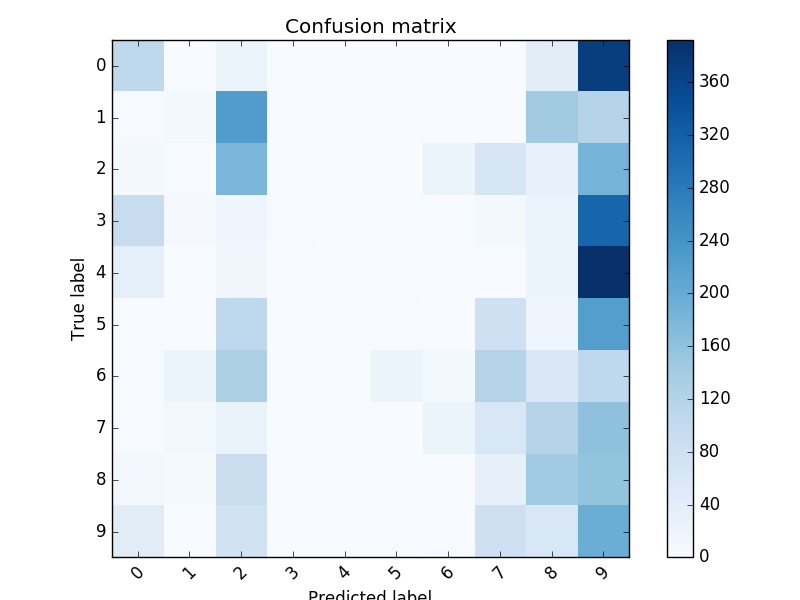
\includegraphics[width=0.5\textwidth]{handpose_plot_20p_c9}
		\caption{Confusion matrix for an SVM trained on HoG features of 20 participants (6 participants in test set).}
		\label{hand_estimation_cm}
	\end{figure}
	\begin{table}
		\begin{tabular}{c|c|c|c|c}
			c1 vs c3 & c2 vs c4 & c0 vs c7 & c0 vs c5 & c3 vs c4 \\ 
			\hline 
			98\% & 86\% & 94\% & 84\% & 91\% \\ 
		\end{tabular} 
		\caption{Classification accuracies for different 1-vs-1 classifiers trained on 8 participants (3 participants in test set).}
		\label{hand_estimation_1vs1}
	\end{table}
	Although the classification accuracy of an SVM with HoG features is significantly better then random with more then 30\%, it is not good enough to be practically relevant. The confusion matrix in Figure \ref{hand_estimation_cm} displays the classification errors of a classifier trained on 20 participants (6 participants in the test set) and HoG features. There does not seem to be any logically explainable confusion. To further investigate our thesis that some of the classes should be easy to distinguish based on the appearance of the hands on the steering wheel, we trained a few 1-vs-1 classifiers. As is illustrated in Table \ref{hand_estimation_1vs1}, they did achieve a very good accuracy. 
	
	
\subsection{HoG Landmarks}
\begin{figure}[h]
	\centering
	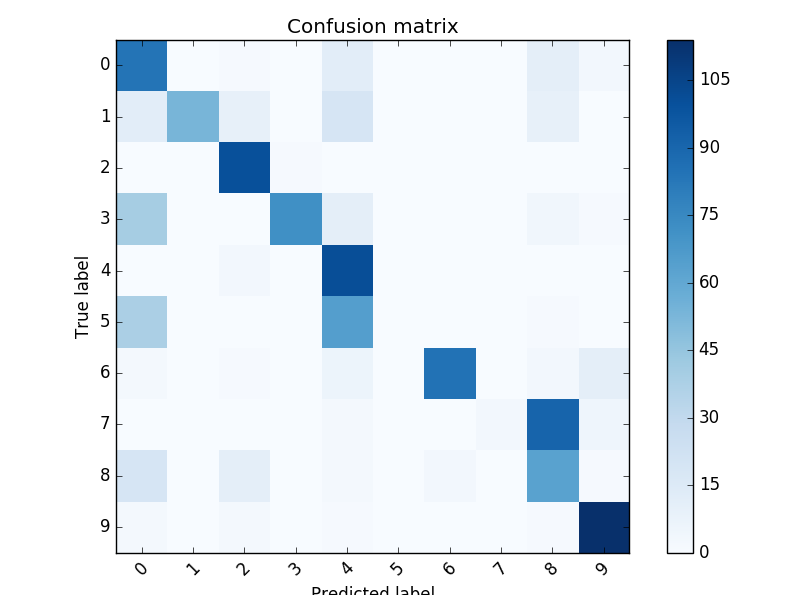
\includegraphics[width=0.5\textwidth]{mult_HOG/4c0123456789matComparable}
	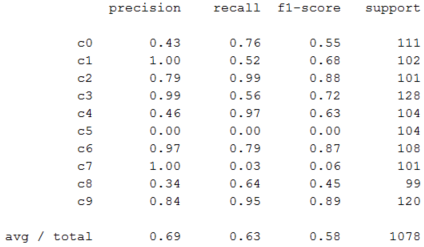
\includegraphics[width=0.4\textwidth]{mult_HOG/4c0123456789repComparable}
	\caption{\textit{Above.} Confusion matrix for an SVM trained on HoG Landmarks of 4 participants and evaluated on 1 test participant. \textit{Below.} Textual report of the mentioned setting}
	\label{Landmarks_4all}
\end{figure}

The initial results already outperform previous approaches as can be seen from Figure \ref{Landmarks_4all}  with almost 70\% average precision. However, there are some things to be noted. The recall for classes c5(operating the radio) and c7(reaching behind) is critically low (0.0 and 0.3 respectively) which leads us to believe that the Landmarks are very loosely defined and, thus, cannot be properly recognized. This has a big impact of course in the average precision and recall. 

\begin{figure}[h]
	\centering
	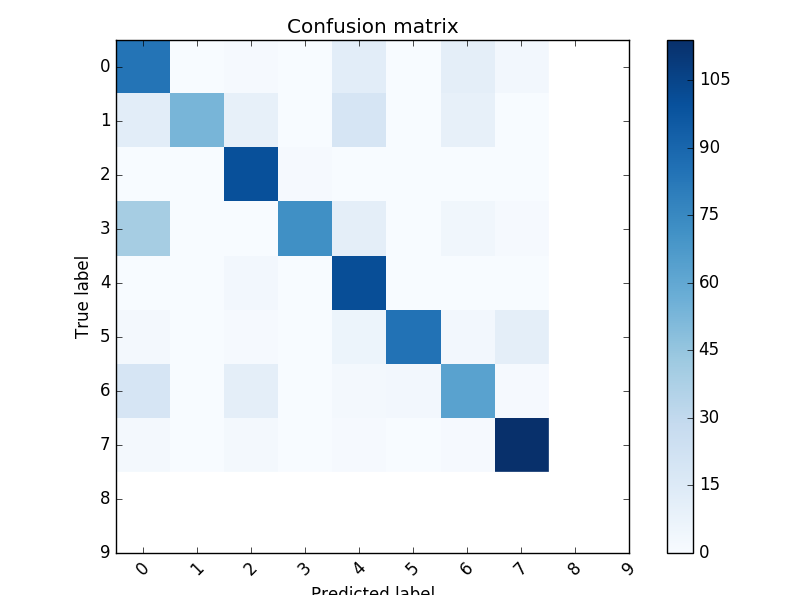
\includegraphics[width=0.5\textwidth]{mult_HOG/4c01234689matComparable}
	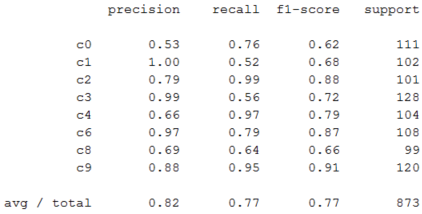
\includegraphics[width=0.4\textwidth]{mult_HOG/4c01234689repComparable}
	\caption{\textit{Above.} Confusion matrix for an SVM trained on HoG Landmarks of 4 participants and evaluated on 1 test participant. Classes c5 and c7 have been omitted and classes c6, c8 and c9 have been shifted to the left. \textit{Below.} Textual report of the mentioned setting}
	\label{Landmarks_4no5no7}
\end{figure}

The question might follow: how well does the approach work for the classes whose Landmarks are effectively recognized?. By removing both classes c5 and c7, average precision and recall are both improved over 13\% as can be appreciated from Figure \ref{Landmarks_4no5no7}. 

Now if we take a look at class c4(taking on the phone left hand), we see that recall is quite good at 97\% whereas its precision is only 66\% indicating possibly multiple false positives as show in Figure \ref{Landmarks_false_detection}. This is most likely due to the labeling of this particular landmark, since when talking on the phone with the left hand, part of the face is inside the bounding box and occluding part of the phone.


\begin{figure}[h]
	\centering
	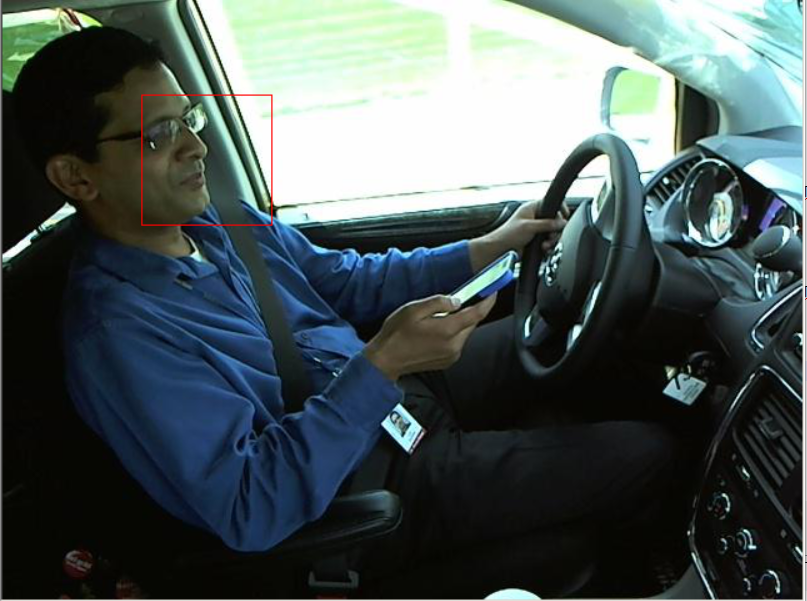
\includegraphics[width=0.5\textwidth]{mult_HOG/talk_phone_left}
	\caption{False positive. A detector identifies the use of the phone for talking with the left hand, where in reality the left hand is holding the wheel. }
	\label{Landmarks_false_detection}
\end{figure}

Class c1 (texting with the right hand) on the other hand has comparably low recall, at at 52\%, but 100\% precision which indicates that this is a strong feature and that even though there are very few false positives, there may remain almost half of the images without detecting the phone on the hand. The same can be said about class c3 (texting with the left hand) This may be due to the angle in which the person is using the phone. Another possibility is of course that other detectors are producing false positives, and thus interfering with the decision.

Other classes such as c0(safe driving) and c8(hair and makeup) have arguably lower both precision and recall than some of the ther better recognized classes. While it is not completely obvious what happens here, most likely the landmarks characteristic of these classes are not sufficient, to determine i.e. their landmarks are present in several other classes, as in the head facing front, however the it could also be possible that some of the landmarks are not recognized and some times they give false positives.


\begin{figure}[h]
	\centering
	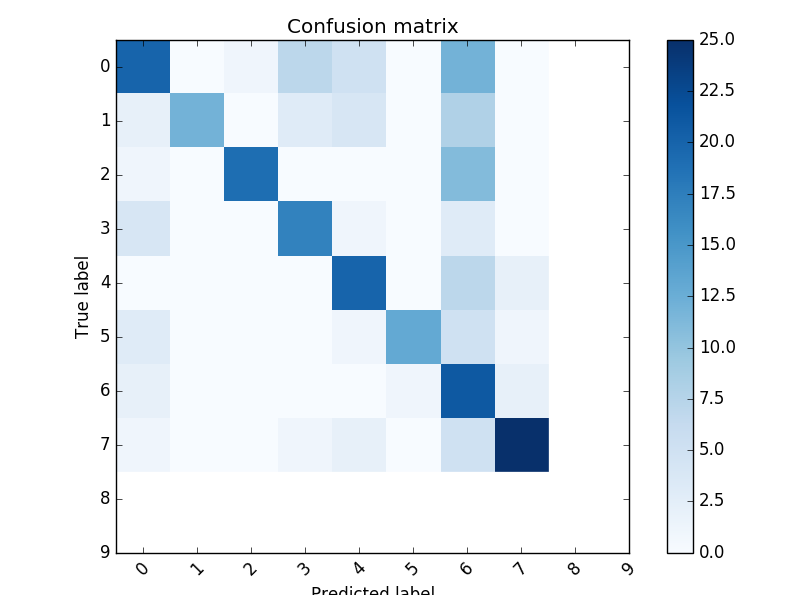
\includegraphics[width=0.5\textwidth]{mult_HOG/4c01234689matTest}
	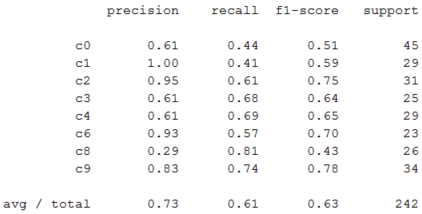
\includegraphics[width=0.4\textwidth]{mult_HOG/4c01234689repTest}
	\caption{\textit{Above.} Confusion matrix for an SVM trained on HoG Landmarks of 4 participants and evaluated on several test participants. Classes c5 and c7 have been omitted and classes c6, c8 and c9 have been shifted to the left. \textit{Below.} Textual report of the mentioned setting}
	\label{Landmarks_4no5no7test}
\end{figure}

Finally since there is much bias in testing only against one participant, we have tested also several images from the Testset. These images were randomly picked and manually labeled with the right class, however since this required manual work, only a handful of images, 242 in 8 classes, were selected. In Figure \ref{Landmarks_4no5no7test} we can see the results of this. The performance is still comparable with the aforementioned outcomes, but interesting to note is that the overall recall dropped much (15\%) and the precision particularly from class c8 dropped remarkably low (29\% vs 69\% before). As can be seen from the confusion matrix many images of, in general, all classes were wrongly predicted to be class c8. As mentioned before, this may be due to classes not particularly well defined by landmarks, landmarks not being detected in the images, or many false positives from class c8 for which we would need to improve the robustness of the detectors.

\section{Conclusion}
Concluding from our experiments we think that it is save to say that you can not easily achieve with Convolutional Neural Network comparable performance using only classic computer vision algorithms. It might be a good idea to combine both aproaches for example by using a bodypose estimation like we mentioned in the proposed methods part using neural networks to complement our current approach. Although you would have to experiment with this to see if it is worth it.

Assuming you do not have the computational limitations we had, we think that traditional methods are difficult to use for such a complex task, mainly because they need to be highly customized to ''work together'' seamlessly and it is probably not worth spending this much time experimenting when you could just use a CNN and achieve extremely high precisions immediately. 


\section{Future Work}
Regarding the future work, we think that the approach we have, can still be optimized a lot by experimenting with combining what we have right now and trying different parameters for everything. The biggest problem is to get features that describe everything important well. Additionally implementing a body-pose estimation like mentioned in our proposed methods will most likely benefit our classification, because it could be used to describe the arms position. This combined with the hand- and headpose-estimation would basically cover all the important bodyparts to distinguish between all the classes. To achieve this we would probably have to invest in new hardware to increase our computational power.




%%%%%%%%% REFERENCES

{\small
\bibliographystyle{ieee}
\bibliography{egbib}
}

\end{document}
